% Especificaciones del tamaño de letra, tamaño de hoja, márgenes, librerias, etc.
\documentclass[12pt, letterpaper]{article}
\usepackage[english]{babel}
\usepackage[utf8]{inputenc}
\usepackage[T1]{fontenc}
\usepackage{amsmath}
\usepackage{graphicx}
\usepackage{subcaption}
\usepackage{hyperref}
\usepackage{url}
\usepackage{amssymb}
\usepackage{float}
\usepackage[margin=1in]{geometry}
\renewcommand{\baselinestretch}{1.5}

% Enlace Bibliografía
\usepackage{csquotes}
\usepackage[notes,backend=biber]{biblatex-chicago}
\addbibresource{referencias.bib}

% Titulo, autores, fecha.
\title{Práctica \#2: Análisis de Tensión de Von Mises}
\author{Carlos Vásquez 1155057}

% Inicio del documento
\begin{document}
\maketitle
\section*{Introducción}

Anteriormente, en la práctica \#1, se analizó la resistencia que tenía una barra de aluminio ante una fuerza de tensión que actuaba a lo largo de ella. La manera de calcular cuál fue el esfuerzo máximo fue a través de la aplicación de una fuerza conocida a nuestra barra de aluminio de dimenciones previamente medidas. Estos cálculos son efectivos, sin embargo es importante reconocer las limitaciones físicas que se nos presentan al utilizar materiales en la naturaleza. Los materiales en la realidad no son isotrópicos u homogéneos, lo cual puede afectar su resistencia a las fuerzas que apliquemos, es por eso que optamos por realizar las pruebas.

A pesar de estas limitantes, los cálculos teóricos son herramientas útiles para la toma de decisiones apropiadas. En la industria puede ser muy tardado realizar estos análisis a mano, por lo que se opta por realizar simulaciones de los materiales, con las dimensiones y características de las piezas en cuestión.
\subsubsection*{Diagramas de esfurzo-deformación}
Cuando a un objeto que se encuentra en un estado de equilibrio inicial se le aplican fuerzas, el cuerpo se deforma correspondientemente hasta que llega a un nuevo estado de \textbf{equilibrio mecánico} o estado de deformación. Las fuerzas internas en el cuerpo resultan de un campo de fuerzas, como la gravedad, y las fuerzas superficiales aplicadas al cuerpo en cuestión. 

La relación entre las fuerzas externas (normalmente llamadas "fuerzas de esfuerzo") y la deformación del cuerpo se llama relación esfuerzo-deformación. Esta relación representa propiedades del material que compone al cuerpo y también son conocidas como ecuaciones constitutivas.\autocite{sim16}

\begin{figure}[H]
	\centering
	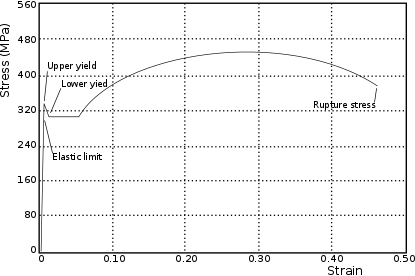
\includegraphics[width=0.9\textwidth]{ssdiagramsteel.png}
	\caption{Diagrama de esfuerzo-deformación del \textit{acero suave} con distintos puntos de interés.}
\end{figure}

\section*{Desarrollo}

El análisis se llevó a cabo en el software CATIA, en el cual se modeló una barra de acero similar a un ejercicio teórico visto en clase. El plano de la barra se describe en la figura 2, junto con sus dimensiones. Una vez hecho el plano, también se definió una longitud para la barra, de 120 pulgadas. Con todas estas características, pusimos a prueba nuestra barra de acero y realizamos el análisis correspondiente para calcular la tensión de von Mises. En la figura 3 se muestra una tabla que describe las propiedades del material utilizado.

\begin{figure}[H]
	\centering
	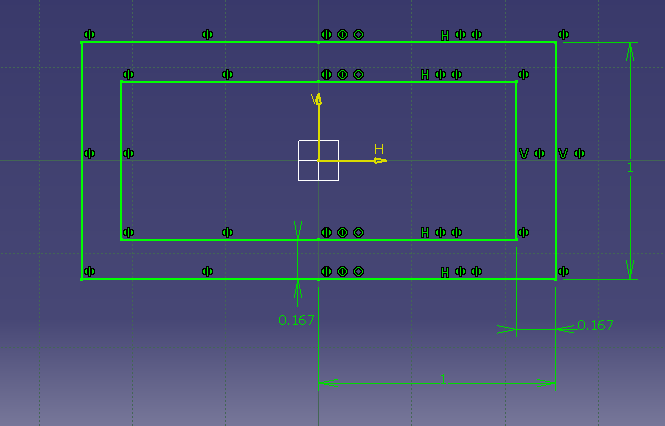
\includegraphics[width=0.9\textwidth]{dimensions.png}
	\caption{Sección transversal de la barra de acero modelada en CATIA, con las dimensiones descritas en pulgadas.}
\end{figure}

\begin{figure}[H]
	\centering
	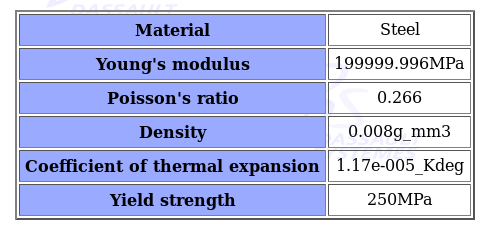
\includegraphics[width=0.75\textwidth]{properties.png}
	\caption{Distintas propiedades del material utilizado.}
\end{figure}
La fuerza que se aplicó a nuestra barra fue una fuerza de compresión de 15,000 N, esta carga es la que utilizaremos posteriormente para realizar los cálculos. Teniendo en cuenta todos estos datos, el análisis hecho por el software de CATIA se muestra en las siguientes figuras.

\begin{figure}[H]
	\centering
	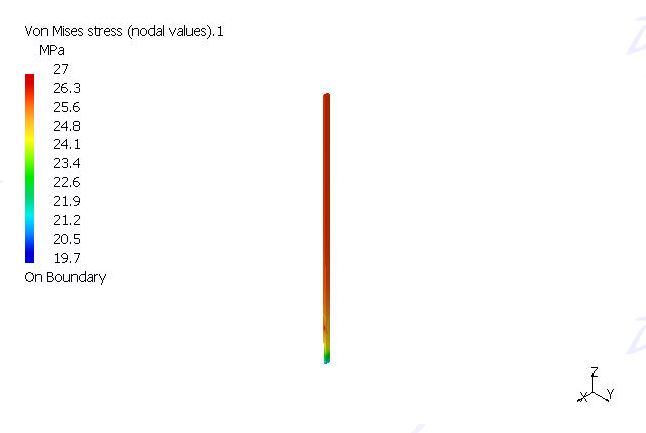
\includegraphics[width=\textwidth]{analisis.png}
	\caption{Gradiente de esfuerzo presentado en la barra de acero, es posible observar que el mayor esfuerzo ocurre en la parte superior de la barra, donde se aplica la fuerza de compresión.}
\end{figure}
Se aprecia un esfuerzo máximo de aproximadamente 27 MPa.
\section*{Cálculos}

Para realizar los cálculos será necesario conocer el área sobre la cual se aplica la fuerza de compresión y la magnitud de esta fuerza. Gracias a la figura 1 podemos calcular el área de la barra de acero. A su vez, ya sabemos la fuerza que será ejercida sobre la barra, la cual será de 15,000 N a compresión.

Para calcular el área, obtendremos las respectivas áreas del rectángulo exterior y el rectángulo interior, para posteriormente restarlas y obtener el área de la sección transversal de la barra. Las medidas mostradas en la figura 1 se convertirán al sistema métrico para ser consistentes con los cálculos a continuación.

\begin{equation*}
\begin{split}
	Dimensiones\ del\ rectángulo\ exterior&: 0.0508\ m \times 0.0254\ m\\
	Dimensiones\ del\ rectángulo\ interior&: 0.0423333\ m \times 0.0169333\ m
\end{split}
\end{equation*}

\begin{equation}
	\begin{split}
	A_{ext}	&= 0.0508\ m \times 0.0254\ m\\
	A_{ext} &= 1.29032 \times 10^{-3}\ m^2\\
	A_{int} &= 0.0423333\ m \times 0.0169333\ m\\
	A_{int} &= 7.168425 \times 10^{-4}\ m^2
	\end{split}
\end{equation}

\begin{equation}
	\begin{split}
	A_T &= A_{ext} - A_{int}\\
	&= (1.29032 \times 10^{-3})\ m - (7.168425 \times 10^{-4}\ m)\\
		&\approx5.73478 \times 10^{-4}\ m^2
	\end{split}
\end{equation}

A partir de los resultados de las ecuaciones 1 y 2, podemos calcular el esfuerzo normal que experimentará la superficie al aplicar la carga de 15,000 N. Se asume que la distribución de fuerzas es uniforme.

\begin{equation}
	\begin{split}
		\sigma &= \frac{P}{A}\\
		&= \frac{15,000\ N}{5.73478 \times 10^{-4}\ m^2}\\
		&\approx 26,156,190.82\ Pa\\
		&\boxed{\approx 26.2\ MPa}
	\end{split}
\end{equation}

\section*{Conclusión}

Como podemos apreciar, los cálculos realizados por el software CATIA y los cálculos realizados en la sección anterior son muy parecidos, sin embargo es necesario remarcar que los cálculos hechos en este reporte son muy sencillos y asumen muchas condiciones ideales. CATIA es un software más profesional y éste toma en cuenta muchas otras variables como la longitus, distintas relaciones, el tipo de material, etcétera.

A pesar de estas limitaciones que hemos impuesto sobre nuestros cálculos, ambos resultados son bastante cercanos y podemos llegar a la conclusión de que el software es bastante acertado al momento de realizar estas simulaciones. La simulación que realiza CATIA se realiza en cuestión de segundos, mientras que aquellas hechas por nosotros son mucho más tardadas y puede existir bastante espacio para el error humano.

Gracias a esta práctica fue mucho más fácil visualizar cómo una fuerza afecta a un objeto, al igual que la deformación que éste sufre por dicho esfuerzo. Es muy interesante ver la teoría en acción y así poder experimentar los fenómenos físicos que se dan en la práctica.
%%%%%  Bib
\renewcommand\refname{Referencias}
\printbibliography
\end{document}
